% Created by tikzDevice version 0.12.3.1 on 2021-05-23 20:22:01
% !TEX encoding = UTF-8 Unicode
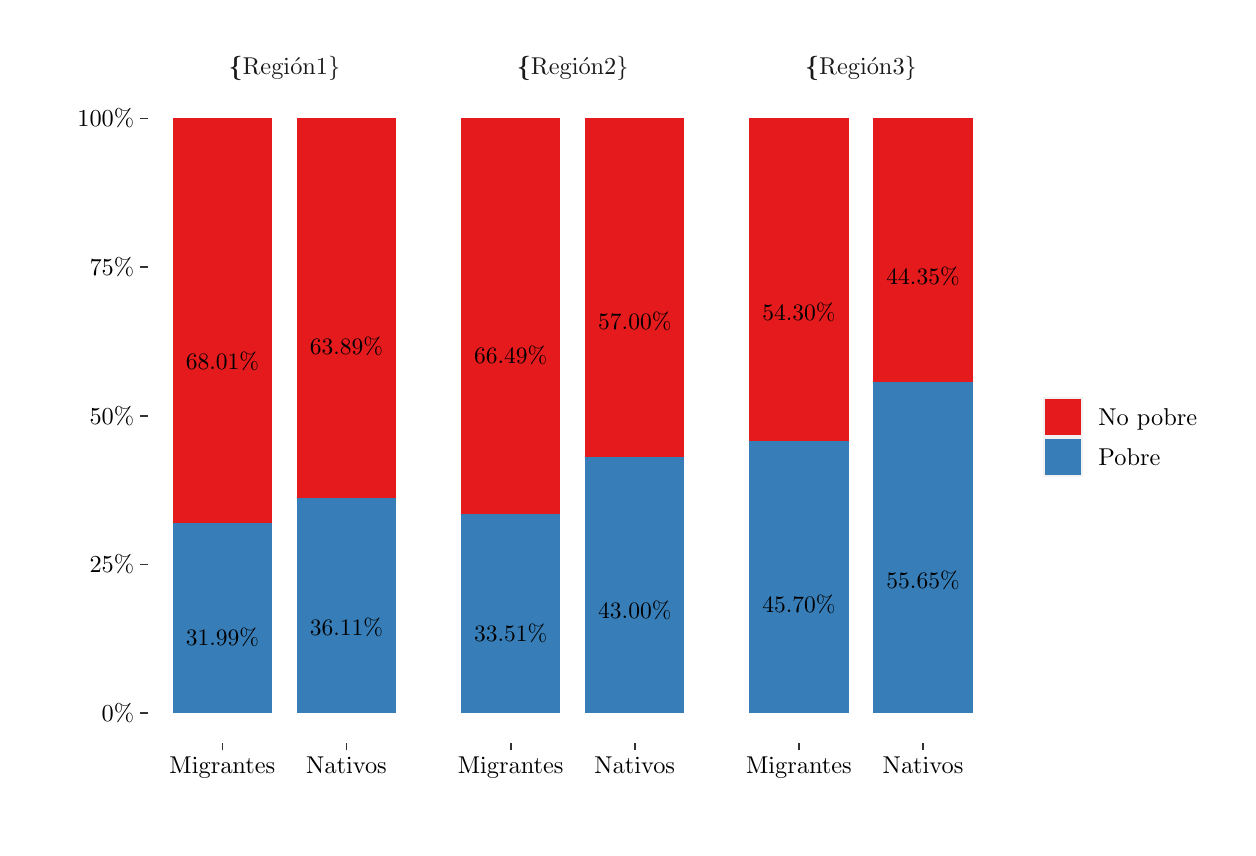
\begin{tikzpicture}[x=1pt,y=1pt]
\definecolor{fillColor}{RGB}{255,255,255}
\path[use as bounding box,fill=fillColor,fill opacity=0.00] (0,0) rectangle (433.62,289.08);
\begin{scope}
\path[clip] (  0.00,  0.00) rectangle (433.62,289.08);
\definecolor{drawColor}{RGB}{255,255,255}
\definecolor{fillColor}{RGB}{255,255,255}

\path[draw=drawColor,line width= 0.6pt,line join=round,line cap=round,fill=fillColor] (  0.00,  0.00) rectangle (433.62,289.08);
\end{scope}
\begin{scope}
\path[clip] ( 43.44, 30.69) rectangle (142.12,267.01);
\definecolor{drawColor}{RGB}{255,255,255}

\path[draw=drawColor,line width= 0.3pt,line join=round] ( 43.44, 68.28) --
	(142.12, 68.28);

\path[draw=drawColor,line width= 0.3pt,line join=round] ( 43.44,121.99) --
	(142.12,121.99);

\path[draw=drawColor,line width= 0.3pt,line join=round] ( 43.44,175.70) --
	(142.12,175.70);

\path[draw=drawColor,line width= 0.3pt,line join=round] ( 43.44,229.41) --
	(142.12,229.41);

\path[draw=drawColor,line width= 0.6pt,line join=round] ( 43.44, 41.43) --
	(142.12, 41.43);

\path[draw=drawColor,line width= 0.6pt,line join=round] ( 43.44, 95.14) --
	(142.12, 95.14);

\path[draw=drawColor,line width= 0.6pt,line join=round] ( 43.44,148.85) --
	(142.12,148.85);

\path[draw=drawColor,line width= 0.6pt,line join=round] ( 43.44,202.56) --
	(142.12,202.56);

\path[draw=drawColor,line width= 0.6pt,line join=round] ( 43.44,256.27) --
	(142.12,256.27);

\path[draw=drawColor,line width= 0.6pt,line join=round] ( 70.35, 30.69) --
	( 70.35,267.01);

\path[draw=drawColor,line width= 0.6pt,line join=round] (115.20, 30.69) --
	(115.20,267.01);
\definecolor{fillColor}{RGB}{228,26,28}

\path[fill=fillColor] ( 52.41,110.15) rectangle ( 88.29,256.27);
\definecolor{fillColor}{RGB}{55,126,184}

\path[fill=fillColor] ( 52.41, 41.43) rectangle ( 88.29,110.15);
\definecolor{fillColor}{RGB}{228,26,28}

\path[fill=fillColor] ( 97.26,119.00) rectangle (133.15,256.27);
\definecolor{fillColor}{RGB}{55,126,184}

\path[fill=fillColor] ( 97.26, 41.43) rectangle (133.15,119.00);
\definecolor{drawColor}{RGB}{0,0,0}

\node[text=drawColor,anchor=base,inner sep=0pt, outer sep=0pt, scale=  0.85] at ( 70.35,165.66) {68.01{\%}};

\node[text=drawColor,anchor=base,inner sep=0pt, outer sep=0pt, scale=  0.85] at ( 70.35, 65.98) {31.99{\%}};

\node[text=drawColor,anchor=base,inner sep=0pt, outer sep=0pt, scale=  0.85] at (115.20,170.97) {63.89{\%}};

\node[text=drawColor,anchor=base,inner sep=0pt, outer sep=0pt, scale=  0.85] at (115.20, 69.52) {36.11{\%}};
\end{scope}
\begin{scope}
\path[clip] (147.62, 30.69) rectangle (246.29,267.01);
\definecolor{drawColor}{RGB}{255,255,255}

\path[draw=drawColor,line width= 0.3pt,line join=round] (147.62, 68.28) --
	(246.29, 68.28);

\path[draw=drawColor,line width= 0.3pt,line join=round] (147.62,121.99) --
	(246.29,121.99);

\path[draw=drawColor,line width= 0.3pt,line join=round] (147.62,175.70) --
	(246.29,175.70);

\path[draw=drawColor,line width= 0.3pt,line join=round] (147.62,229.41) --
	(246.29,229.41);

\path[draw=drawColor,line width= 0.6pt,line join=round] (147.62, 41.43) --
	(246.29, 41.43);

\path[draw=drawColor,line width= 0.6pt,line join=round] (147.62, 95.14) --
	(246.29, 95.14);

\path[draw=drawColor,line width= 0.6pt,line join=round] (147.62,148.85) --
	(246.29,148.85);

\path[draw=drawColor,line width= 0.6pt,line join=round] (147.62,202.56) --
	(246.29,202.56);

\path[draw=drawColor,line width= 0.6pt,line join=round] (147.62,256.27) --
	(246.29,256.27);

\path[draw=drawColor,line width= 0.6pt,line join=round] (174.53, 30.69) --
	(174.53,267.01);

\path[draw=drawColor,line width= 0.6pt,line join=round] (219.38, 30.69) --
	(219.38,267.01);
\definecolor{fillColor}{RGB}{228,26,28}

\path[fill=fillColor] (156.59,113.42) rectangle (192.47,256.27);
\definecolor{fillColor}{RGB}{55,126,184}

\path[fill=fillColor] (156.59, 41.43) rectangle (192.47,113.42);
\definecolor{fillColor}{RGB}{228,26,28}

\path[fill=fillColor] (201.44,133.81) rectangle (237.32,256.27);
\definecolor{fillColor}{RGB}{55,126,184}

\path[fill=fillColor] (201.44, 41.43) rectangle (237.32,133.81);
\definecolor{drawColor}{RGB}{0,0,0}

\node[text=drawColor,anchor=base,inner sep=0pt, outer sep=0pt, scale=  0.85] at (174.53,167.62) {66.49{\%}};

\node[text=drawColor,anchor=base,inner sep=0pt, outer sep=0pt, scale=  0.85] at (174.53, 67.29) {33.51{\%}};

\node[text=drawColor,anchor=base,inner sep=0pt, outer sep=0pt, scale=  0.85] at (219.38,179.85) {57.00{\%}};

\node[text=drawColor,anchor=base,inner sep=0pt, outer sep=0pt, scale=  0.85] at (219.38, 75.44) {43.00{\%}};
\end{scope}
\begin{scope}
\path[clip] (251.79, 30.69) rectangle (350.46,267.01);
\definecolor{drawColor}{RGB}{255,255,255}

\path[draw=drawColor,line width= 0.3pt,line join=round] (251.79, 68.28) --
	(350.46, 68.28);

\path[draw=drawColor,line width= 0.3pt,line join=round] (251.79,121.99) --
	(350.46,121.99);

\path[draw=drawColor,line width= 0.3pt,line join=round] (251.79,175.70) --
	(350.46,175.70);

\path[draw=drawColor,line width= 0.3pt,line join=round] (251.79,229.41) --
	(350.46,229.41);

\path[draw=drawColor,line width= 0.6pt,line join=round] (251.79, 41.43) --
	(350.46, 41.43);

\path[draw=drawColor,line width= 0.6pt,line join=round] (251.79, 95.14) --
	(350.46, 95.14);

\path[draw=drawColor,line width= 0.6pt,line join=round] (251.79,148.85) --
	(350.46,148.85);

\path[draw=drawColor,line width= 0.6pt,line join=round] (251.79,202.56) --
	(350.46,202.56);

\path[draw=drawColor,line width= 0.6pt,line join=round] (251.79,256.27) --
	(350.46,256.27);

\path[draw=drawColor,line width= 0.6pt,line join=round] (278.70, 30.69) --
	(278.70,267.01);

\path[draw=drawColor,line width= 0.6pt,line join=round] (323.55, 30.69) --
	(323.55,267.01);
\definecolor{fillColor}{RGB}{228,26,28}

\path[fill=fillColor] (260.76,139.61) rectangle (296.64,256.27);
\definecolor{fillColor}{RGB}{55,126,184}

\path[fill=fillColor] (260.76, 41.43) rectangle (296.64,139.61);
\definecolor{fillColor}{RGB}{228,26,28}

\path[fill=fillColor] (305.61,160.99) rectangle (341.49,256.27);
\definecolor{fillColor}{RGB}{55,126,184}

\path[fill=fillColor] (305.61, 41.43) rectangle (341.49,160.99);
\definecolor{drawColor}{RGB}{0,0,0}

\node[text=drawColor,anchor=base,inner sep=0pt, outer sep=0pt, scale=  0.85] at (278.70,183.33) {54.30{\%}};

\node[text=drawColor,anchor=base,inner sep=0pt, outer sep=0pt, scale=  0.85] at (278.70, 77.76) {45.70{\%}};

\node[text=drawColor,anchor=base,inner sep=0pt, outer sep=0pt, scale=  0.85] at (323.55,196.16) {44.35{\%}};

\node[text=drawColor,anchor=base,inner sep=0pt, outer sep=0pt, scale=  0.85] at (323.55, 86.31) {55.65{\%}};
\end{scope}
\begin{scope}
\path[clip] ( 43.44,267.01) rectangle (142.12,283.58);
\definecolor{drawColor}{gray}{0.10}

\node[text=drawColor,anchor=base,inner sep=0pt, outer sep=0pt, scale=  0.88] at ( 92.78,272.26) {\textbf{\{}Región1{\}}};
\end{scope}
\begin{scope}
\path[clip] (147.62,267.01) rectangle (246.29,283.58);
\definecolor{drawColor}{gray}{0.10}

\node[text=drawColor,anchor=base,inner sep=0pt, outer sep=0pt, scale=  0.88] at (196.95,272.26) {\textbf{\{}Región2{\}}};
\end{scope}
\begin{scope}
\path[clip] (251.79,267.01) rectangle (350.46,283.58);
\definecolor{drawColor}{gray}{0.10}

\node[text=drawColor,anchor=base,inner sep=0pt, outer sep=0pt, scale=  0.88] at (301.12,272.26) {\textbf{\{}Región3{\}}};
\end{scope}
\begin{scope}
\path[clip] (  0.00,  0.00) rectangle (433.62,289.08);
\definecolor{drawColor}{gray}{0.20}

\path[draw=drawColor,line width= 0.6pt,line join=round] ( 70.35, 27.94) --
	( 70.35, 30.69);

\path[draw=drawColor,line width= 0.6pt,line join=round] (115.20, 27.94) --
	(115.20, 30.69);
\end{scope}
\begin{scope}
\path[clip] (  0.00,  0.00) rectangle (433.62,289.08);
\definecolor{drawColor}{RGB}{0,0,0}

\node[text=drawColor,anchor=base,inner sep=0pt, outer sep=0pt, scale=  0.88] at ( 70.35, 19.68) {Migrantes};

\node[text=drawColor,anchor=base,inner sep=0pt, outer sep=0pt, scale=  0.88] at (115.20, 19.68) {Nativos};
\end{scope}
\begin{scope}
\path[clip] (  0.00,  0.00) rectangle (433.62,289.08);
\definecolor{drawColor}{gray}{0.20}

\path[draw=drawColor,line width= 0.6pt,line join=round] (174.53, 27.94) --
	(174.53, 30.69);

\path[draw=drawColor,line width= 0.6pt,line join=round] (219.38, 27.94) --
	(219.38, 30.69);
\end{scope}
\begin{scope}
\path[clip] (  0.00,  0.00) rectangle (433.62,289.08);
\definecolor{drawColor}{RGB}{0,0,0}

\node[text=drawColor,anchor=base,inner sep=0pt, outer sep=0pt, scale=  0.88] at (174.53, 19.68) {Migrantes};

\node[text=drawColor,anchor=base,inner sep=0pt, outer sep=0pt, scale=  0.88] at (219.38, 19.68) {Nativos};
\end{scope}
\begin{scope}
\path[clip] (  0.00,  0.00) rectangle (433.62,289.08);
\definecolor{drawColor}{gray}{0.20}

\path[draw=drawColor,line width= 0.6pt,line join=round] (278.70, 27.94) --
	(278.70, 30.69);

\path[draw=drawColor,line width= 0.6pt,line join=round] (323.55, 27.94) --
	(323.55, 30.69);
\end{scope}
\begin{scope}
\path[clip] (  0.00,  0.00) rectangle (433.62,289.08);
\definecolor{drawColor}{RGB}{0,0,0}

\node[text=drawColor,anchor=base,inner sep=0pt, outer sep=0pt, scale=  0.88] at (278.70, 19.68) {Migrantes};

\node[text=drawColor,anchor=base,inner sep=0pt, outer sep=0pt, scale=  0.88] at (323.55, 19.68) {Nativos};
\end{scope}
\begin{scope}
\path[clip] (  0.00,  0.00) rectangle (433.62,289.08);
\definecolor{drawColor}{RGB}{0,0,0}

\node[text=drawColor,anchor=base east,inner sep=0pt, outer sep=0pt, scale=  0.88] at ( 38.49, 38.40) {0{\%}};

\node[text=drawColor,anchor=base east,inner sep=0pt, outer sep=0pt, scale=  0.88] at ( 38.49, 92.11) {25{\%}};

\node[text=drawColor,anchor=base east,inner sep=0pt, outer sep=0pt, scale=  0.88] at ( 38.49,145.82) {50{\%}};

\node[text=drawColor,anchor=base east,inner sep=0pt, outer sep=0pt, scale=  0.88] at ( 38.49,199.53) {75{\%}};

\node[text=drawColor,anchor=base east,inner sep=0pt, outer sep=0pt, scale=  0.88] at ( 38.49,253.24) {100{\%}};
\end{scope}
\begin{scope}
\path[clip] (  0.00,  0.00) rectangle (433.62,289.08);
\definecolor{drawColor}{gray}{0.20}

\path[draw=drawColor,line width= 0.6pt,line join=round] ( 40.69, 41.43) --
	( 43.44, 41.43);

\path[draw=drawColor,line width= 0.6pt,line join=round] ( 40.69, 95.14) --
	( 43.44, 95.14);

\path[draw=drawColor,line width= 0.6pt,line join=round] ( 40.69,148.85) --
	( 43.44,148.85);

\path[draw=drawColor,line width= 0.6pt,line join=round] ( 40.69,202.56) --
	( 43.44,202.56);

\path[draw=drawColor,line width= 0.6pt,line join=round] ( 40.69,256.27) --
	( 43.44,256.27);
\end{scope}
\begin{scope}
\path[clip] (  0.00,  0.00) rectangle (433.62,289.08);
\definecolor{fillColor}{RGB}{255,255,255}

\path[fill=fillColor] (361.46,121.29) rectangle (428.12,176.41);
\end{scope}
\begin{scope}
\path[clip] (  0.00,  0.00) rectangle (433.62,289.08);
\definecolor{fillColor}{gray}{0.95}

\path[fill=fillColor] (366.96,141.24) rectangle (381.42,155.69);
\end{scope}
\begin{scope}
\path[clip] (  0.00,  0.00) rectangle (433.62,289.08);
\definecolor{fillColor}{RGB}{228,26,28}

\path[fill=fillColor] (367.67,141.95) rectangle (380.70,154.98);
\end{scope}
\begin{scope}
\path[clip] (  0.00,  0.00) rectangle (433.62,289.08);
\definecolor{fillColor}{gray}{0.95}

\path[fill=fillColor] (366.96,126.79) rectangle (381.42,141.24);
\end{scope}
\begin{scope}
\path[clip] (  0.00,  0.00) rectangle (433.62,289.08);
\definecolor{fillColor}{RGB}{55,126,184}

\path[fill=fillColor] (367.67,127.50) rectangle (380.70,140.53);
\end{scope}
\begin{scope}
\path[clip] (  0.00,  0.00) rectangle (433.62,289.08);
\definecolor{drawColor}{RGB}{0,0,0}

\node[text=drawColor,anchor=base west,inner sep=0pt, outer sep=0pt, scale=  0.88] at (386.92,145.44) {No pobre};
\end{scope}
\begin{scope}
\path[clip] (  0.00,  0.00) rectangle (433.62,289.08);
\definecolor{drawColor}{RGB}{0,0,0}

\node[text=drawColor,anchor=base west,inner sep=0pt, outer sep=0pt, scale=  0.88] at (386.92,130.98) {Pobre};
\end{scope}
\end{tikzpicture}
